\documentclass[9pt]{exam} 
\addpoints

\usepackage{cmbright}
\usepackage{amsmath, amssymb} 
\usepackage[a4paper, margin=1in]{geometry}
\usepackage{tcolorbox} 
\usepackage{tikz}

\tcbset{colback=black!5!white}

\begin{document}

\textbf{Name:} \dotfill

\

Show all your working on a separate page. Plot the objects on the grid to the right as you go along.

\vspace{-4mm}

\begin{questions}

\begin{minipage}[t]{0.6\textwidth}
\fullwidth{Santa Claus flies in two segments through points $A(4,0)$, $B(-4,0)$ to $C(0,6)$.}


\question[3] Calculate the gradient of $[BC]$. \newline
\emph{Points for the formula, substitution of values, and the result.}
%\fillwithdottedlines{21mm}


\question[3] Calculate the angle that Santa turns through at $B$.
%\fillwithdottedlines{21mm}

\fullwidth{Rudolph the Red-Nosed Reindeer is sat at $D$, the centre of gravity of $\triangle ABC$, watching Santa fly around him. \newline \emph{The center of gravity of a triangle is where the medians intersect.}
}

\question[3] Determine the gradient-intercept form of the median $d_1$ of $\triangle ABC$ passing through $B$.
%\fillwithdottedlines{35mm}

\question[3] Calculate the coordinates of Rudolf. \hfill \emph{Explain logic!}
%\fillwithdottedlines{35mm}

\fullwidth{Santa realizes he forgot a gift at point $E$ in the third quadrant.}

\question[3] $[EF]$ is parallel to $[AB]$ such that $\triangle DEF$ has area 48. If $\overline{DE} = \overline{DF} = 10$, determine the coordinates of $E$ and $F$.
%\fillwithdottedlines{\stretch{1}}

\question[3] Calculate the distance $\overline{CE}$ in exact values.
%\fillwithdottedlines{10mm}

\end{minipage}
\hfill
\begin{minipage}[t]{0.35\textwidth}
\vspace{0mm}

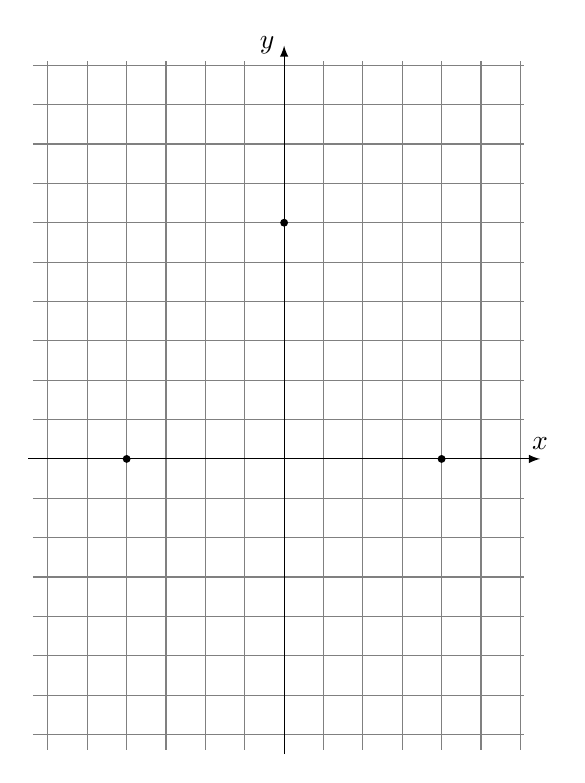
\begin{tikzpicture}[scale=0.5]

\draw[gray] (-6.0,-7,1) grid (6.1,10.1);

% Axes
\draw[-latex] (-6.5,0) -- (6.5,0) node[above]{$x$};
\draw[-latex] (0,-7.5) -- (0,10.5) node[left]{$y$};

\fill[black] (4,0) circle (0.1);
\fill[black] (-4,0) circle (0.1);
\fill[black] (0,6) circle (0.1);

\end{tikzpicture}
\end{minipage}	

\question[3] Determine the geometric object with equation $x^2 + y^2 - 18y  + 80 = 0$.

\question[2] The point $C$ is the center of an equilateral triangle $XYZ$ with vertex $X$ at $(0,9)$. Sketch $\triangle XYZ$ on the grid.

\question[2] \textbf{Bonus.} Decorate your tree !

\question[2] \textbf{Bonus.} Calculate the coordinates of $Y$ and $Z$.


\end{questions}

\begin{tcolorbox}
\textbf{Name of marker:}

\begin{center}
\gradetable[h][questions]
\end{center}
\end{tcolorbox}

\end{document}
